\documentclass{standalone}
\usepackage{tikz}
\usepackage{pgfplots}
\begin{document}
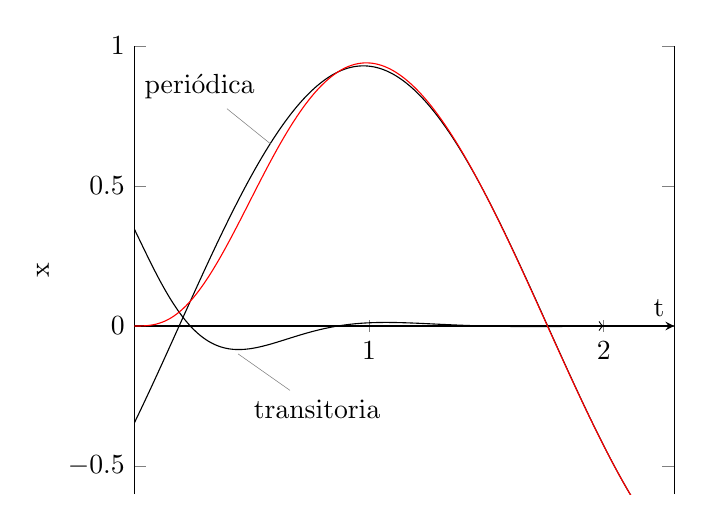
\begin{tikzpicture}
\begin{axis}[
	xmin = 0,	
	xmax = 2.3,
	axis x line = middle,
	%axis y line = center,
	ymin = -0.6,
	ymax = 1,
	ylabel=x,
	xlabel=t,
	xtick={1,2},
	xticklabels={$1$, $2$},
	domain=0:2.3
]
\draw [->] (0,0) -- (2,0);
\addplot [samples=500] plot ({\x},{0.17241 * (-2 * cos(2 * deg(\x)) + 5 * sin(2 * deg(\x)))});
\node[coordinate,  pin={100:{peri\'{o}dica}}] at (axis cs: 0.58,0.65) {};
\addplot [samples=500] plot ({\x},{0.06896 * (exp(-3 * \x))* (5 * cos(5 * deg(\x)) - 2 * sin(5 * deg(\x)))});
\node[ pin={-70:{transitoria}}] at (axis cs:0.4,-0.075){};
\addplot [color=red, samples=500] plot ({\x},{(0.17241 * (-2 * cos(2 * deg(\x)) + 5 * sin(2 * deg(\x)))) + ( 0.06896 * (exp(-3 * \x))* (5 * cos(5 * deg(\x)) - 2 * sin(5 * deg(\x)))});
\end{axis}

\end{tikzpicture}
\end{document}